\chapter{Gemista}
\label{ch:gemista}
\index{meal}
\index{rice}
\index{vegetables}
\index{meat}

\marginnote{
    \textbf{Makes 8+ servings} \\
    Prep time: 45 minutes \\
    Cook time: 1 hour \\
    \vspace*{\baselineskip}
    
    ? g ground beef, extra lean \\
    ? long grain rice, rinsed \\
    6 medium-sized tomatoes \\
    2 red bell peppers \\
    2 green bell peppers \\
    2 garlic cloves \\
    1 cup olive oil \\
    1 cup fresh parsley, chopped \\
    1 cup fresh mint, chopped \\
    1 can tomato juice, Heinz (540 ml) \\
    1 large onion, thinly chopped \\
    4 red potatoes, peeled and cut into wedges \\
    Breadcrumbs \\
    Salt, pepper and oregano \\
    Grated Pecorino cheese, Chelmos Greek
}

\textit{Tomatoes and Peppers stuffed with meat and rice}

Family member: Mom

\newthought {Gemista} are vegetables stuffed with rice, minced meat and herbs cooked with potatoes in a tomato sauce. They are usually made with tomatoes, bell peppers, zucchini, eggplants... My grandmother even stuffed potatoes because I didn't like vegetables as a child! \textgreek{Καλή όρεξη}!

\begin{marginfigure}
  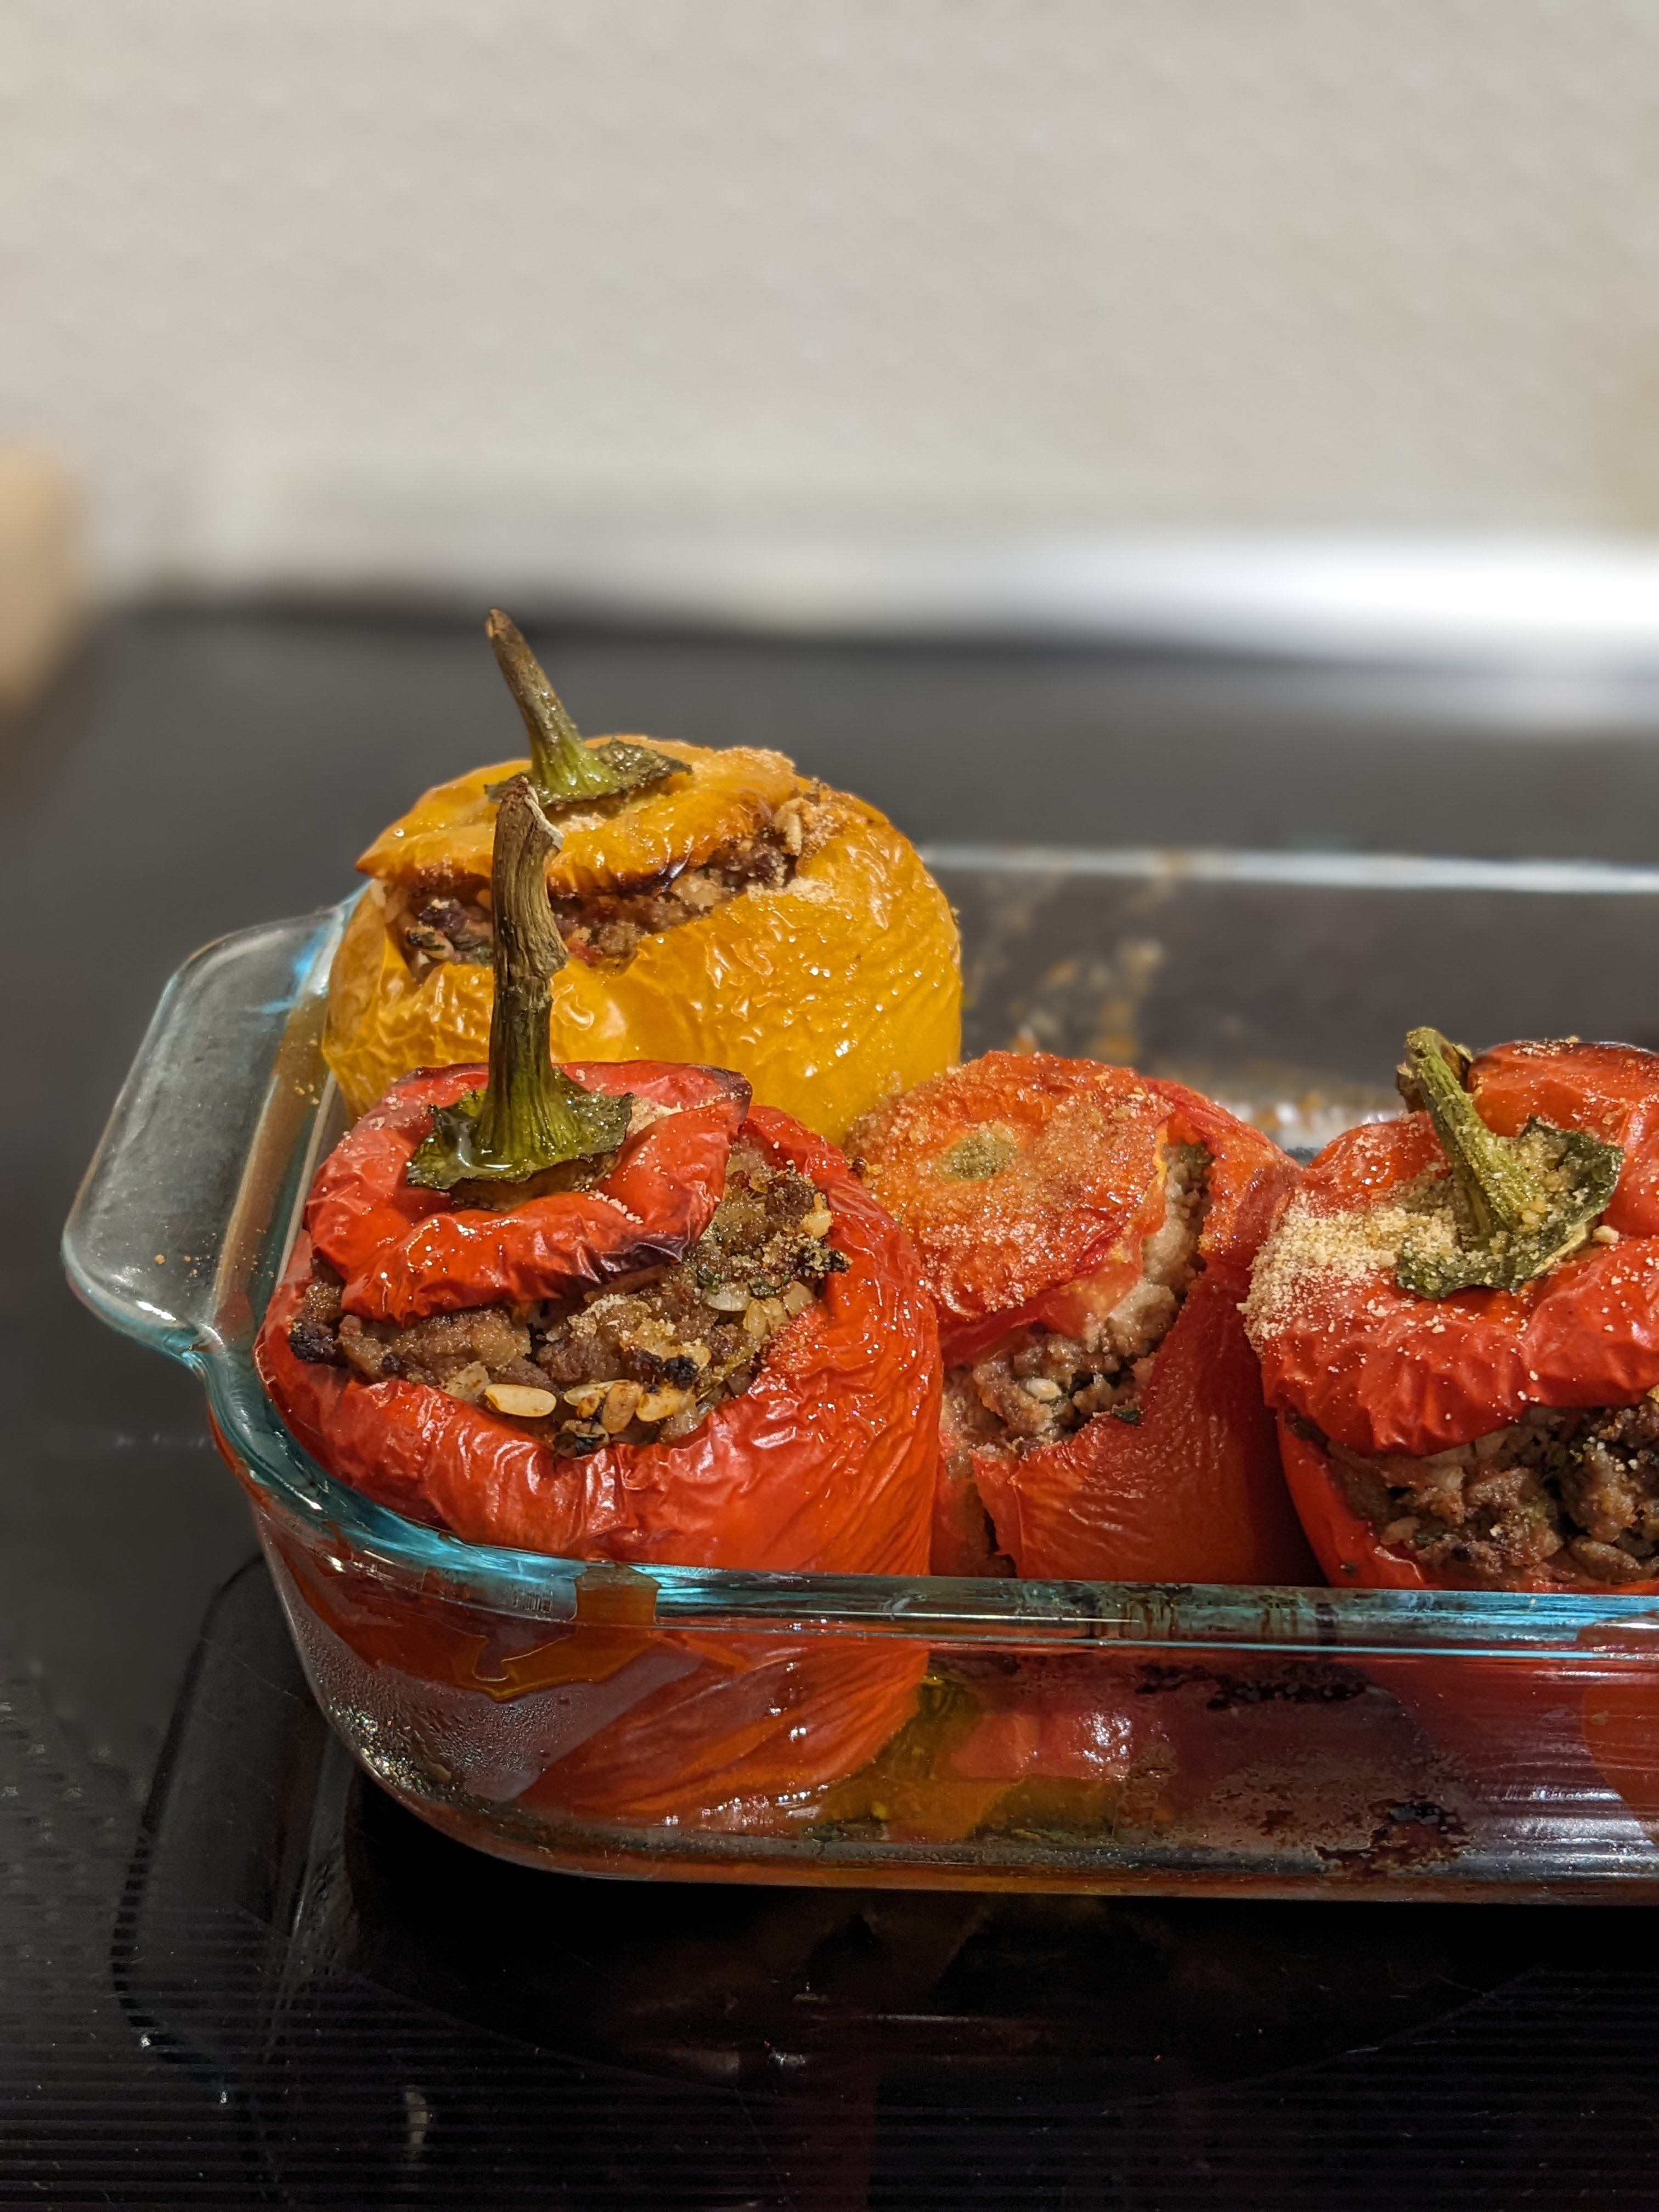
\includegraphics[width=60mm]{monanteras/images/Cooked gemista.jpg}
\end{marginfigure}

\begin{enumerate}
    \item Preheat oven to 350\degree F and grease a 9X13-inch ovenproof dish with Pam spray.
    \item Wash the tomatoes and remove the stems. Slice the tops off each tomato, leaving a bit of flesh attached. Carefully remove the flesh out of each tomato and place it into a bowl. Place each one of the tomatoes into the prepared baking dish and place their tops aside.
    \item Cut the top of the peppers, clean the inside of each and place them in the baking dish, place their tops aside.
    \item Heat 1/2 cup of olive oil in a pot and cook the onion. Once softened, add the garlic and stir well. Add the minced meat, rice, parsley and mint, and stir well. Season with salt and pepper, and cook until the meat has browned. Add the insides of the tomatoes and 1/2 can of Heinz tomato juice. Stir well.
    \item Using a spoon, stuff the tomatoes and the peppers until a little below the rim and cover with their tops. Arrange the sliced potatoes around the \textgreek{Γεμιστά}.
    \item Pour the remaining 1/2 can of tomato juice as well as 1/2 cup water in the pan. Drizzle the other 1/2 cup olive oil over the tomatoes and potatoes. Season with salt, pepper and oregano. Add some breadcrumbs and grated Pecorino cheese on the tops.
    \item Bake in the preheated oven uncovered for 60-70 minutes, or until the tomatoes are golden on top. The potatoes should be easily pierced with a knife.
\end{enumerate}
